
\chapter{Implementation of DAS visualization application}\label{txt.implementation}

This chapter provides an implementation overview of the DAS visualization application. Based on the previous chapters we put everything together and create an application for data processing and visualization. The whole application consists of two main parts a Python back-end and a JavaScript front-end. 

\section{Python back-end application implementation}\label{txt.implementation.python}

Back-end is written in programming language Python3.10. To run the application it is advisable to create virtual environment and install all the dependencies in that environment. Installation steps can be found in Attachments \ref{atach:dependencies}. The application consists of multiple files as can be seen in \ref{dir:filestructure.python}. 

\bigskip
Python back-end file structure:

{\small
%
\label{dir:filestructure.python}
\dirtree{%.
.1 optasense\_visualizer.
.2 app.py\DTcomment{Python script to run the application}.
.2 requirements.txt\DTcomment{Dependencies}
.2 src/\DTcomment{Folder with source files}.
.3 file\_reader.py\DTcomment{Opens and reads HDF5 files}.
.3 message\_classes.py\DTcomment{Data classes for incoming messages}.
.3 optasense\_server.py\DTcomment{Back-end part of application}.
.3 range\_parser.py\DTcomment{Functions for parsing channels}.
.3 spectral\_analysis.py\DTcomment{Functions for processing data}.
.3 streaming.py \DTcomment{Managing data streaming}.
}
}
\bigskip


The application is started by calling \verb|python3 app.py --port 8001|. Everything runs inside with use of \textit{asyncio} library. The \textit{app.py} file parses arguments with the use of \textit{argparse} library. Only argument is optional \textit{port} argument, default value is 8001, which is later used by \textit{websocket}. Websocket uses \textit{async for} waiting for messages from the client side. Incoming messages are in the JSON format. Every message has a \textit{type} which determines which message is incoming. Messages are parsed using \textit{MessageParser} class, which implements a \textit{factory object}.
\textit{Factory} object is one of the most used object oriented design patterns. It creates objects without revealing the logic to the client. The only implemented method is \verb|parse()| which reads the type and then it creates one of the message classes and returns it. Each message corresponds to its own message class. For ease of programming \textit{dataclasses} module was used. It provides functions and a decorator for automatic generation of special methods (\verb|__init__()| or \verb|__repr__()|). There are 6 message dataclasses \textit{InitApp}, \textit{FindFiles}, \textit{OpenFile}, \textit{Streaming}, \textit{Properties} and \textit{ChannelSelection}, see Figure \ref{fig:uml}. When the message parsing fails it raises an \verb|UnknownMessageException|. The exception is thrown away as we do not want to terminate execution every time an incorrect message is received.

Message classes and the factory object \verb|MessageFactory| are located in the \textit{message\_classes.py} file with an \textit{Exception} class \verb|UnknownMessageException|.

\begin{figure}
    \centering
    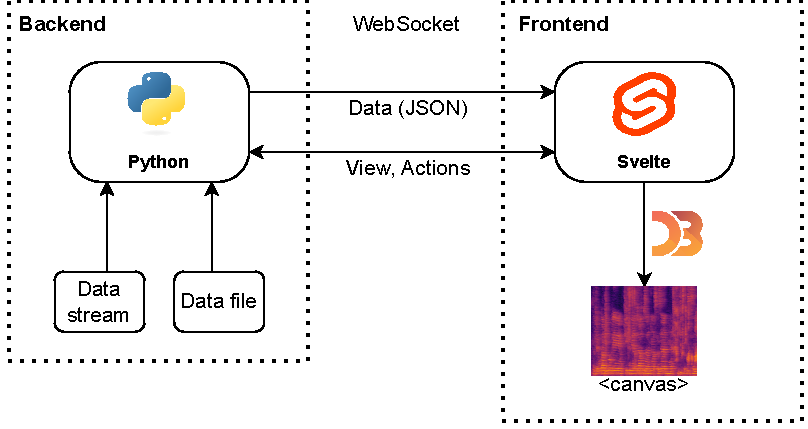
\includegraphics{obrazky/appstack.drawio.pdf}
    \caption{UML diagram of the back-end}
    \label{fig:uml}
\end{figure}

An example of incoming message from the client, received by the server:
\begin{verbatim}
{
    'type': 'path',
    'path': '/Users/user/Documents/',
    'suffix': '.h5'
}
\end{verbatim}

Next the MessageFactory checks the message \verb|type| - \textit{"path"} corresponds to \textit{FindFiles} class and returns it. The message class is than saved as a server state. Each message class then has its own \textit{if} statement with its own behaviour.

\textit{FindFiles} is the first message sent from the client 

\section{Program implementation of HDF5 to WAV}\label{lab:hdftowav}\label{txt.implementation.wav}

The goal of this part of project is to create an application for reading data from the \ac{das} system and converting the data to the \verb|.wav| audio file format.

For the implementation of this application, the Python\footnote{\url{https://www.python.org/}} programming language was chosen. Python is a~great language for scientific use, data visualization, and graph plotting, which is the goal. The biggest advantage comes from the availability of scientific libraries. The opening of \verb |.h5| files is done with \verb|h5py| library\footnote{\url{https://www.h5py.org/}}. For working with dataset data types \verb|numpy|\footnote{\url{https://numpy.org/}} library is used. The function for interpolating arrays to a~certain range is also used \verb|interp|. Lastly, to convert the signal data to \verb|.wav| audio format \verb|scipy| library is used specifically \verb|io| module function \verb|wavfile|. To read all options and input arguments, the \verb|argparse| library is used\footnote{\url{https://docs.python.org/3/library/argparse.html}}.

\subsection{Reading HDF5 file}\label{txt.implementation.reading}

The sample file recorded in the OptaSense ODH-F is in HDF5 file format. As \ac{hdf} files have a~user-defined structure on the application layer and in the binary form it is hard to say what is actually in the file. To better understand the contents of the \verb|.h5| file, \verb|h5dump| was performed and a conversion to JSON\footnote{\url{https://www.json.org/json-en.html}} was also performed by the \verb|h5tojson| program\footnote{\url{https://hdf5-json.readthedocs.io/en/latest/tools/h5json.html}}. The JSON file is quite large in size - the original HDF5 file is only \qty{52,7}{MB} and the JSON file is \qty{946,6}{MB}. The dump text file is half the size and provides the same information, but the datasets are harder to understand, but the whole file is only half the size of the JSON file at ``only'' \qty{420}{MB}. The JSON format is much easier to read. The structure of the file is divided into 3 parts:

\begin{itemize}
    \item \textit{apiVersion} - 1.1.1 version of API
    \item \textit{datasets} - Contain all the datasets organized by their UUID\footnote{Universally unique identifier} that are defined in the groups section. There is also an \textit{alias} that is in the format of a Unix-based system path, for example, \verb|"/Acquisition/Raw[0]/Custom/SampleCount"|. There are also other properties that define the shape and type of stored data. In this case, the properties are shown in the table \ref{tab:file_details}.
    \item \textit{groups} - Groups are named by a UUID. The group object has:
        \begin{itemize}
            \item \textit{alias} - Unix-like name; the first is root ``/'' group
            \item \textit{attributes} - define the type, name, and shape of the value of the attribute which is a string \verb|979bb2ac-99bf-4cb5-b410-5c16cd7872dc|
            \item \textit{links} - links to other groups that create a treelike structure. The link object contains the class of a link (e.g. H5L\_TYPE\_HARD for hard link), the \textit{collection} property telling that it is a group and the name of the group. The group object also contains other important metadata, such as measurement settings. All important details are given in the table \ref{tab:file_details}
        \end{itemize}
\end{itemize}

There is a~library for reading \ac{hdf} files written in Python called \verb|h5py|. To read the contents of the file, a~function was created called \verb|get_dataset_path()| which recursively looks for all groups, according to their name provided by the \verb|.keys()| method, in the dataset. The result of this function is propagated through recursion and saved in Python \verb|set()| built-in type. The user can then choose which one is the right dataset to use because there is probably more than one dataset. The user can save the string and use it as an argument when calling the program. This saves time in searching for the contents of the file. 

This is the data structure of the DAS file from the OptaSense Interrogator:

\bigskip
DAS output file structure in \ac{hdf} format
{\small
%
\label{dir:filestructure}
\dirtree{%.
.1 /\DTcomment{root}.
.2 Acquisition\DTcomment{Recorded data}.
.3 Custom\DTcomment{Empty}.
.3 Raw[0]\DTcomment{HDF5 group (3 members)}.
.4 Custom\DTcomment{HDF5 group (1 members)}.
.5 SampleCount\DTcomment{HDF5 dataset, shape (332032,), type "<i8">}.
.4 RawData[0]\DTcomment{HDF5 dataset, shape (100, 332032), type "<i2">}.
.4 RawDataTime\DTcomment{HDF5 dataset, shape (332032,), type "<i8">}.
}
}
\bigskip

The type of explanation in \ref{dir:filestructure} is \verb|i8|, which is \verb|numberpy.int64|. \verb|SampleCount| contains numbering of all samples, \verb|RawDataTime| contains time, and \verb|RawData[0]| contains useful sensor data that we need to read in the next steps; see \ref{txt.design.datapprocessing}. More details are provided in Table \ref{tab:file_details}.

All important HDF5 attributes are shown in the table \ref{tab:file_details}, it contains metadata information about the datasets, data dimensions, number of channels, kinds of filters used, time information, length of pulses, laser wavelength, and more. Some properties can be derived from those in the table. The capture duration can be calculated from the start and end of the capture, which is \qty{10,376}{\second}.

\subsection{Data processing for converting raw HDF5 data to WAV}\label{txt.implementation.processing}

The useful data have 100 channels with \textit{N} samples, in this example \qty{332032}{samples} saved in \verb|/Acquisition/Raw[0]/RawData[0]|, see the file structure in \ref{dir:filestructure}. The function \verb|scipy.io.wavfile.write()| is used to save samples to a file and the data need some more processing before the function can be called. After the data are read from the file, it is saved into \verb|samples| variable of type \verb|numpy.array| it is then processed in 4 steps as preparation for saving into \verb|.wav| file. The steps are:

\begin{enumerate}
    \item \textbf{Channel selection} - only channel one can be selected.
    \item \textbf{Data interpolation} - The original data have a bad value range from -24838 to -30758, triggering an exception when writing the data into a \verb|.wav| file. The \verb|numpy.interp()|\footnote{\url{https://numpy.org/doc/stable/reference/generated/numpy.interp.html}} function interpolates the data into the range of the maximum and minimum values specified in this case by the \qty{16}{bit} PCM\footnote{Pulse Code Modulation}, which can be written to WAV file by \verb|wavfile| module.
    \item \textbf{Resampling} - as the data are recorded at a certain sampling frequency, in this case, \qty{10}{\kHz}, resampling by the function \verb|scipy.signal.resample() |\footnote{\url{https://docs.scipy.org/doc/scipy/reference/generated/scipy.signal.resample.html}} is necessary. The right number of samples is calculated by the formula \ref{formula:sampling}.
    \item \textbf{Retyping} - the resampled data need to be in the correct format and since the interpolation was done in the range of \verb|int16| the output type of choice is the same \verb|samples.astype(np.int16)|.
\end{enumerate}

\begin{equation}
    \label{formula:sampling}
    numSamples = \frac{44100}{fs.len(samples)}
\end{equation}


\begin{table}[]
    \centering
    \begin{tabular}{|c|c|c|c|}
    \hline
    \textbf{Data type} & \textbf{Minimum value} & \textbf{Maximum value} & \textbf{WAV format} \\
    \hline
    float32 & -1.0 & +1.0 & 32-bit floating-point \\ \hline
    int32 & -2147483648 & +2147483647 & 32-bit PCM \\ \hline
    int16 & -32768 & +32767 & 16-bit PCM \\ \hline
    uint8 & 0 & 255 & 8-bit PCM \\
    \hline
    \end{tabular}
    \caption{WAV compatible types}
    \label{tab:my_label}
\end{table}





\section{Svelte}\label{txt.implementation.svelte}
\subsection{Svelte components}\label{txt.implementation.components}
\subsection{Svelte stores}\label{txt.implementation.stores}

